\documentclass[11pt,a4paper]{article}

% Page geometry
\usepackage[margin=1in]{geometry}

% Fonts and encoding
\usepackage[T1]{fontenc}
\usepackage[utf8]{inputenc}
\usepackage{lmodern}
\usepackage{microtype}

% Math
\usepackage{amsmath,amssymb,amsthm}
\usepackage{bm}

% Colors
\usepackage[dvipsnames,svgnames,x11names]{xcolor}

% Code listings
\usepackage{listings}
\usepackage{inconsolata}

% Boxes for problems
\usepackage[most]{tcolorbox}

% Graphics
\usepackage{graphicx}
\usepackage{tikz}
\usetikzlibrary{positioning}

% Tables
\usepackage{booktabs}
\usepackage{array}

% Hyperlinks
\usepackage{hyperref}
\hypersetup{
    colorlinks=true,
    linkcolor=RoyalBlue,
    urlcolor=RoyalBlue,
    citecolor=RoyalBlue
}

% Headers
\usepackage{fancyhdr}
\pagestyle{fancy}
\fancyhf{}
\fancyhead[L]{\small SmulGrad: Building Automatic Differentiation from Scratch}
\fancyhead[R]{\small \thepage}
\renewcommand{\headrulewidth}{0.4pt}

% Section formatting
\usepackage{titlesec}
\titleformat{\section}{\Large\bfseries}{\thesection}{1em}{}
\titleformat{\subsection}{\large\bfseries}{\thesubsection}{1em}{}
\titleformat{\subsubsection}{\normalsize\bfseries}{\thesubsubsection}{1em}{}

% Custom colors matching Stanford style
\definecolor{problemorange}{RGB}{204, 119, 34}
\definecolor{codebg}{RGB}{248, 248, 248}
\definecolor{codegreen}{RGB}{0, 128, 0}
\definecolor{codepurple}{RGB}{128, 0, 128}
\definecolor{codeblue}{RGB}{0, 0, 180}
\definecolor{codered}{RGB}{180, 0, 0}
\definecolor{codegray}{RGB}{128, 128, 128}

% Code listing style
\lstdefinestyle{pythonstyle}{
    language=Python,
    basicstyle=\ttfamily\small,
    backgroundcolor=\color{codebg},
    keywordstyle=\color{codeblue}\bfseries,
    stringstyle=\color{codered},
    commentstyle=\color{codegreen}\itshape,
    numberstyle=\tiny\color{codegray},
    breaklines=true,
    breakatwhitespace=true,
    tabsize=4,
    showstringspaces=false,
    frame=single,
    framerule=0.5pt,
    rulecolor=\color{gray!50},
    xleftmargin=2em,
    framexleftmargin=1.5em,
    numbers=left,
    numbersep=8pt,
    morekeywords={self, True, False, None, as, with, yield, lambda, assert},
    emph={Value, Tensor, Node, Executor, Linear, SGD},
    emphstyle=\color{codepurple},
}

\lstdefinestyle{pythonsimple}{
    language=Python,
    basicstyle=\ttfamily\small,
    backgroundcolor=\color{codebg},
    keywordstyle=\color{codeblue}\bfseries,
    stringstyle=\color{codered},
    commentstyle=\color{codegreen}\itshape,
    breaklines=true,
    breakatwhitespace=true,
    tabsize=4,
    showstringspaces=false,
    frame=single,
    framerule=0.5pt,
    rulecolor=\color{gray!50},
    morekeywords={self, True, False, None, as, with, yield, lambda, assert},
    emph={Value, Tensor, Node, Executor, Linear, SGD},
    emphstyle=\color{codepurple},
}

\lstdefinestyle{bashstyle}{
    language=bash,
    basicstyle=\ttfamily\small,
    backgroundcolor=\color{codebg},
    keywordstyle=\color{codeblue},
    breaklines=true,
    frame=single,
    framerule=0.5pt,
    rulecolor=\color{gray!50},
}

\lstset{style=pythonstyle}

% Problem box environment
\newtcolorbox{problembox}[2][]{
    enhanced,
    colback=white,
    colframe=problemorange,
    coltitle=black,
    fonttitle=\bfseries,
    title={Problem (#1): #2},
    attach boxed title to top left={yshift=-2mm, xshift=4mm},
    boxed title style={
        colback=white,
        colframe=white,
    },
    top=4mm
}

% Deliverable environment
\newcommand{\deliverable}[1]{%
    \textbf{Deliverable:} #1%
}

% Inline code
\newcommand{\code}[1]{\texttt{\small #1}}

% Parameter description
\newcommand{\param}[2]{\code{#1}: \texttt{#2}}

% Points indicator
\newcommand{\points}[1]{\hfill\textbf{(#1 points)}}

\begin{document}

% Title
\begin{center}
    {\LARGE\bfseries SmulGrad: Building Automatic Differentiation from Scratch}\\[1em]
    {\large A Hands-On Learning Assignment}\\[0.5em]
    {\normalsize Inspired by Stanford CS336 and Karpathy's micrograd}
\end{center}

\vspace{1em}

\tableofcontents

\newpage

%==============================================================================
\section{Overview}
%==============================================================================

Automatic differentiation (autodiff) is the backbone of modern deep learning frameworks. Unlike symbolic differentiation (which manipulates mathematical expressions) or numerical differentiation (which approximates derivatives using finite differences), autodiff computes exact derivatives by decomposing computations into elementary operations and applying the chain rule systematically.

In \textbf{reverse-mode autodiff} (also called backpropagation), we:
\begin{enumerate}
    \item Build a computational graph during the forward pass
    \item Traverse this graph backwards to accumulate gradients using the chain rule
\end{enumerate}

This approach is efficient when we have many inputs and few outputs---exactly the case in neural network training where we differentiate a scalar loss with respect to millions of parameters.

\subsection{Learning Objectives}

By completing this assignment, you will:
\begin{itemize}
    \item Understand how computational graphs represent mathematical expressions
    \item Implement the reverse-mode autodiff algorithm from scratch
    \item Handle tensor operations and broadcasting in gradient computation
    \item Build a system capable of training neural networks
\end{itemize}

\subsection{Assignment Structure}

\begin{table}[h]
\centering
\begin{tabular}{clc}
\toprule
\textbf{Part} & \textbf{Topic} & \textbf{Points} \\
\midrule
1 & Scalar Values and Basic Operations & 15 \\
2 & The Backward Pass & 20 \\
3 & More Operations & 15 \\
4 & Tensor Support & 22 \\
5 & Matrix Operations & 17 \\
6 & Neural Network Training & 15 \\
\midrule
& \textbf{Total} & \textbf{104} \\
\bottomrule
\end{tabular}
\end{table}

\subsection{Getting Started}

\begin{lstlisting}[style=bashstyle]
# Install dependencies
uv sync

# Run all tests (most will fail initially)
uv run pytest

# Run tests for a specific part
uv run pytest -k "part1"

# Run a single test
uv run pytest -k "TestValueCreation"
\end{lstlisting}

\subsection{File Structure}

\begin{lstlisting}[style=bashstyle,numbers=none]
smulgrad/
    engine.py            # Value and Tensor classes (Parts 1-5)
    nn.py                # Neural network utilities (Part 6)
tests/
    adapters.py          # Adapter functions connecting your code to tests
    cases/               # Test files (do not modify)
        test_part1_scalar.py
        test_part2_backward.py
        test_part3_ops.py
        test_part4_tensor.py
        test_part5_matrix.py
        test_part6_nn.py
        conftest.py      # Pytest fixtures
\end{lstlisting}

You will implement everything in the \code{smulgrad/} directory:
\begin{itemize}
    \item \code{engine.py}: Your \code{Value} and \code{Tensor} classes (Parts 1--5)
    \item \code{nn.py}: Neural network utilities like \code{softmax}, \code{cross\_entropy}, \code{SGD}, \code{Linear} (Part 6)
\end{itemize}

The tests import your code through adapter functions in \code{tests/adapters.py}. Import directly from your modules, e.g., \code{from smulgrad.engine import Value}.

\newpage
%==============================================================================
\section{Part 1: Scalar Values and Basic Operations}
\points{15}
%==============================================================================

We begin by creating a \code{Value} class that wraps a scalar number and tracks operations performed on it. This is the fundamental building block of our autodiff system.

\subsection{The Value Class}

A \code{Value} object needs to store:
\begin{itemize}
    \item \code{data}: The actual numerical value (a Python float)
    \item \code{grad}: The gradient of some output with respect to this value (initialized to 0.0)
    \item \code{\_prev}: A set of \code{Value} objects that this value depends on (its ``children'' in the computational graph)
    \item \code{\_op}: A string describing how this value was created (e.g., \code{'+'}, \code{'*'}, \code{'relu'})
\end{itemize}

\begin{problembox}[value\_creation]{Create a Value class that stores a scalar value \points{2}}

Your \code{Value} class should support:

\begin{lstlisting}[style=pythonsimple]
v = Value(3.0)
print(v.data)  # 3.0
print(v.grad)  # 0.0
\end{lstlisting}

\deliverable{Implement the adapter \code{create\_value} in \code{tests/adapters.py}. Run \code{uv run pytest -k TestValueCreation} to verify.}
\end{problembox}

\subsection{Addition}

We want to be able to add \code{Value} objects together using Python's \code{+} operator. When we compute \code{c = a + b}, we need to:
\begin{enumerate}
    \item Compute \code{c.data = a.data + b.data}
    \item Record that \code{c} depends on \code{a} and \code{b} (store them in \code{c.\_prev})
    \item Record the operation (\code{c.\_op = '+'})
\end{enumerate}

\begin{problembox}[value\_add]{Implement addition for Value objects \points{2}}

Your implementation should support:

\begin{lstlisting}[style=pythonsimple]
a = Value(2.0)
b = Value(3.0)
c = a + b
print(c.data)  # 5.0
\end{lstlisting}

You should also handle adding a \code{Value} to a plain Python number:

\begin{lstlisting}[style=pythonsimple]
a = Value(2.0)
c = a + 3  # Should work
c = 3 + a  # Should also work (hint: __radd__)
\end{lstlisting}

\deliverable{Implement the adapter \code{run\_add} in \code{tests/adapters.py}. Run \code{uv run pytest -k TestValueAdd} to verify.}
\end{problembox}

\subsection{Multiplication}

\begin{problembox}[value\_mul]{Implement multiplication for Value objects \points{2}}

\begin{lstlisting}[style=pythonsimple]
a = Value(2.0)
b = Value(3.0)
c = a * b
print(c.data)  # 6.0

# Also support scalar multiplication
c = a * 3  # Should work
c = 3 * a  # Should also work
\end{lstlisting}

\deliverable{Implement the adapter \code{run\_mul}. Run \code{uv run pytest -k TestValueMul} to verify.}
\end{problembox}

\subsection{Negation and Subtraction}

\begin{problembox}[value\_neg\_sub]{Implement negation and subtraction \points{3}}

\textbf{Hint:} Subtraction can be implemented in terms of addition and negation: \code{a - b = a + (-b)}

\begin{lstlisting}[style=pythonsimple]
a = Value(5.0)
b = Value(3.0)
print((-a).data)      # -5.0
print((a - b).data)   # 2.0
\end{lstlisting}

\deliverable{Implement the adapters \code{run\_neg} and \code{run\_sub}. Run \code{uv run pytest -k TestValueNegSub} to verify.}
\end{problembox}

\subsection{Power}

\begin{problembox}[value\_pow]{Implement raising a Value to a constant power \points{3}}

\begin{lstlisting}[style=pythonsimple]
a = Value(2.0)
c = a ** 3
print(c.data)  # 8.0
\end{lstlisting}

\textbf{Note:} We only support constant exponents (Python int or float), not \code{Value} exponents.

\deliverable{Implement the adapter \code{run\_pow}. Run \code{uv run pytest -k TestValuePow} to verify.}
\end{problembox}

\subsection{Division}

\begin{problembox}[value\_div]{Implement division \points{3}}

\textbf{Hint:} Division can be implemented using multiplication and power: \code{a / b = a * (b ** -1)}

\begin{lstlisting}[style=pythonsimple]
a = Value(6.0)
b = Value(2.0)
print((a / b).data)  # 3.0
\end{lstlisting}

\deliverable{Implement the adapter \code{run\_div}. Run \code{uv run pytest -k TestValueDiv} to verify.}
\end{problembox}

\newpage
%==============================================================================
\section{Part 2: The Backward Pass}
\points{20}
%==============================================================================

Now comes the core of autodiff: computing gradients via backpropagation. The key insight is that each operation knows how to compute the gradient with respect to its inputs, given the gradient with respect to its output.

\subsection{Understanding the Chain Rule}

For a function composition $y = f(g(x))$, the chain rule tells us:
\begin{equation}
    \frac{dy}{dx} = \frac{dy}{dg} \cdot \frac{dg}{dx}
\end{equation}

In our computational graph:
\begin{itemize}
    \item Each node computes some value
    \item The ``upstream gradient'' is the gradient of the final output with respect to this node
    \item Each node must compute the ``downstream gradient''---the gradient with respect to its inputs
\end{itemize}

For addition $c = a + b$:
\begin{align}
    \frac{\partial c}{\partial a} &= 1 & \frac{\partial c}{\partial b} &= 1
\end{align}
So: \code{a.grad += c.grad * 1}, \code{b.grad += c.grad * 1}

For multiplication $c = a \cdot b$:
\begin{align}
    \frac{\partial c}{\partial a} &= b & \frac{\partial c}{\partial b} &= a
\end{align}
So: \code{a.grad += c.grad * b.data}, \code{b.grad += c.grad * a.data}

\subsection{Local Backward Functions}

Each \code{Value} needs a \code{\_backward} function that propagates gradients to its children. This function should be set when the \code{Value} is created by an operation.

\begin{problembox}[backward\_add]{Implement gradient computation for addition \points{3}}

When you create \code{c = a + b}, you should also define \code{c.\_backward} such that calling it will add to \code{a.grad} and \code{b.grad}.

\deliverable{The test \code{test\_backward\_add} will verify your addition backward pass.}
\end{problembox}

\begin{problembox}[backward\_mul]{Implement gradient computation for multiplication \points{3}}

For $c = a \cdot b$:
\begin{itemize}
    \item \code{a.grad += c.grad * b.data}
    \item \code{b.grad += c.grad * a.data}
\end{itemize}

\deliverable{Run \code{uv run pytest -k TestBackwardMul} to verify.}
\end{problembox}

\begin{problembox}[backward\_ops]{Implement gradients for other operations \points{4}}

Gradients for remaining operations:
\begin{align}
    \text{Negation:} \quad \frac{\partial(-a)}{\partial a} &= -1 \\[0.5em]
    \text{Power:} \quad \frac{\partial(a^n)}{\partial a} &= n \cdot a^{n-1} \\[0.5em]
    \text{Division:} \quad \frac{\partial(a/b)}{\partial a} &= \frac{1}{b}, \quad \frac{\partial(a/b)}{\partial b} = -\frac{a}{b^2}
\end{align}

\deliverable{Run \code{uv run pytest -k TestBackwardOps} to verify.}
\end{problembox}

\subsection{Topological Sort and Full Backward}

To compute all gradients, we need to:
\begin{enumerate}
    \item Build a topological ordering of all nodes (children before parents)
    \item Set the gradient of the output node to 1.0
    \item Call \code{\_backward()} on each node in reverse topological order
\end{enumerate}

\begin{problembox}[backward\_full]{Implement a backward() method that computes all gradients \points{5}}

\begin{lstlisting}[style=pythonsimple]
a = Value(2.0)
b = Value(3.0)
c = a * b
d = c + a
d.backward()

print(a.grad)  # d(d)/d(a) = d(c+a)/da = dc/da + 1 = b + 1 = 4.0
print(b.grad)  # d(d)/d(b) = dc/db = a = 2.0
\end{lstlisting}

\textbf{Key implementation detail:} You need to traverse the graph in reverse topological order. Use depth-first search to build the ordering.

\deliverable{Implement the adapter \code{run\_backward}. Run \code{uv run pytest -k TestBackwardFull} to verify.}
\end{problembox}

\subsection{Gradient Accumulation}

When a value is used multiple times in a computation, its gradient should accumulate.

\begin{problembox}[grad\_accumulation]{Ensure gradients accumulate correctly \points{3}}

\begin{lstlisting}[style=pythonsimple]
a = Value(3.0)
b = a + a  # a is used twice
b.backward()
print(a.grad)  # Should be 2.0, not 1.0
\end{lstlisting}

\deliverable{Run \code{uv run pytest -k TestGradAccumulation} to verify.}
\end{problembox}

\begin{problembox}[grad\_of\_grad]{Second derivatives (bonus) \points{2}}

A powerful property of autodiff is that gradients are themselves computations that can be differentiated. If your implementation is clean, second derivatives should work automatically.

\begin{lstlisting}[style=pythonsimple]
a = Value(2.0)
b = a * a  # b = a^2
b.backward()
# a.grad is now 2*a = 4.0
# If we could differentiate again, d(2a)/da = 2
\end{lstlisting}

\deliverable{Run \code{uv run pytest -k TestGradOfGrad} to verify (bonus).}
\end{problembox}

\newpage
%==============================================================================
\section{Part 3: More Operations}
\points{15}
%==============================================================================

Real neural networks need more than just arithmetic. Let's add activation functions and other operations.

\subsection{ReLU}

The Rectified Linear Unit (ReLU) is defined as:
\begin{equation}
    \text{relu}(x) = \max(0, x)
\end{equation}

Its gradient is:
\begin{equation}
    \frac{d(\text{relu}(x))}{dx} = \begin{cases} 1 & \text{if } x > 0 \\ 0 & \text{otherwise} \end{cases}
\end{equation}

\begin{problembox}[relu]{Implement the ReLU activation function \points{3}}

\begin{lstlisting}[style=pythonsimple]
a = Value(-3.0)
b = a.relu()
print(b.data)  # 0.0

c = Value(3.0)
d = c.relu()
print(d.data)  # 3.0
\end{lstlisting}

\deliverable{Implement the adapter \code{run\_relu}. Run \code{uv run pytest -k TestReLU} to verify.}
\end{problembox}

\subsection{Exponential}

\begin{problembox}[exp]{Implement the exponential function \points{3}}

\begin{lstlisting}[style=pythonsimple]
a = Value(2.0)
b = a.exp()
print(b.data)  # e^2 ~ 7.389
\end{lstlisting}

Gradient: $\frac{d(e^x)}{dx} = e^x$

\deliverable{Implement the adapter \code{run\_exp}. Run \code{uv run pytest -k TestExp} to verify.}
\end{problembox}

\subsection{Natural Logarithm}

\begin{problembox}[log]{Implement the natural logarithm \points{3}}

\begin{lstlisting}[style=pythonsimple]
a = Value(2.0)
b = a.log()
print(b.data)  # ln(2) ~ 0.693
\end{lstlisting}

Gradient: $\frac{d(\ln x)}{dx} = \frac{1}{x}$

\deliverable{Implement the adapter \code{run\_log}. Run \code{uv run pytest -k TestLog} to verify.}
\end{problembox}

\subsection{Hyperbolic Tangent}

\begin{problembox}[tanh]{Implement the hyperbolic tangent \points{3}}

\begin{lstlisting}[style=pythonsimple]
a = Value(1.0)
b = a.tanh()
print(b.data)  # tanh(1) ~ 0.7616
\end{lstlisting}

Gradient: $\frac{d(\tanh x)}{dx} = 1 - \tanh^2(x)$

\textbf{Note:} You can implement tanh using exp: $\tanh(x) = \frac{e^{2x} - 1}{e^{2x} + 1}$, but implementing it directly with its own backward is more numerically stable.

\deliverable{Implement the adapter \code{run\_tanh}. Run \code{uv run pytest -k TestTanh} to verify.}
\end{problembox}

\subsection{Complex Expression Test}

\begin{problembox}[complex\_expr]{Test a complex expression combining multiple operations \points{3}}

\begin{lstlisting}[style=pythonsimple]
a = Value(2.0)
b = Value(3.0)
c = a * b + a ** 2
d = c.relu() - b / a
e = d.tanh()
e.backward()
\end{lstlisting}

\deliverable{Run \code{uv run pytest -k TestComplexExpr} to verify.}
\end{problembox}

\newpage
%==============================================================================
\section{Part 4: Tensor Support}
\points{20}
%==============================================================================

Scalars are great for understanding, but real neural networks operate on tensors. Now we extend our system to support multi-dimensional arrays.

\subsection{The Tensor Class}

Create a \code{Tensor} class that wraps a numpy array instead of a scalar. The structure is similar to \code{Value}:
\begin{itemize}
    \item \code{data}: A numpy ndarray
    \item \code{grad}: Gradient array (same shape as data), initialized to zeros
    \item \code{\_prev}: Set of parent tensors
    \item \code{\_op}: Operation string
    \item \code{\_backward}: Backward function
\end{itemize}

\begin{problembox}[tensor\_creation]{Create a Tensor class \points{2}}

\begin{lstlisting}[style=pythonsimple]
t = Tensor([[1.0, 2.0], [3.0, 4.0]])
print(t.data.shape)  # (2, 2)
print(t.grad.shape)  # (2, 2)
\end{lstlisting}

\deliverable{Implement the adapter \code{create\_tensor}. Run \code{uv run pytest -k TestTensorCreation} to verify.}
\end{problembox}

\subsection{Element-wise Operations}

\begin{problembox}[tensor\_elementwise]{Implement element-wise add and multiply for tensors \points{3}}

\begin{lstlisting}[style=pythonsimple]
a = Tensor([[1.0, 2.0], [3.0, 4.0]])
b = Tensor([[5.0, 6.0], [7.0, 8.0]])
c = a + b
print(c.data)  # [[6, 8], [10, 12]]

d = a * b
print(d.data)  # [[5, 12], [21, 32]]
\end{lstlisting}

The backward pass for element-wise operations:
\begin{itemize}
    \item Addition: gradients pass through unchanged
    \item Multiplication: each element's gradient is multiplied by the corresponding element of the other tensor
\end{itemize}

\deliverable{Implement adapters \code{run\_tensor\_add} and \code{run\_tensor\_mul}. Run \code{uv run pytest -k TestTensorElementwise} to verify.}
\end{problembox}

\subsection{Backward Pass for Tensors}

Just like \code{Value}, your \code{Tensor} class needs a \code{backward()} method to compute gradients through the computational graph.

\begin{problembox}[tensor\_backward]{Implement backward() for Tensor \points{2}}

The backward pass for tensors works identically to scalars:
\begin{enumerate}
    \item Build a topological ordering of all tensors in the graph
    \item Set the gradient of the output tensor to ones (same shape as data)
    \item Call \code{\_backward()} on each tensor in reverse topological order
\end{enumerate}

\begin{lstlisting}[style=pythonsimple]
a = Tensor([[1.0, 2.0], [3.0, 4.0]])
b = Tensor([[5.0, 6.0], [7.0, 8.0]])
c = a + b
c.backward()  # Computes gradients for a and b
print(a.grad)  # [[1, 1], [1, 1]]
\end{lstlisting}

\textbf{Note:} For non-scalar outputs, \code{backward()} should initialize the output gradient to \code{np.ones\_like(self.data)}.

\deliverable{Implement the adapter \code{run\_tensor\_backward}. Run \code{uv run pytest -k TestTensorBackward} to verify.}
\end{problembox}

\subsection{Broadcasting}

NumPy broadcasting allows operations between arrays of different shapes. Your backward pass must handle this correctly by summing gradients along broadcasted dimensions.

\begin{problembox}[tensor\_broadcast]{Handle broadcasting in backward pass \points{4}}

\begin{lstlisting}[style=pythonsimple]
a = Tensor([[1.0, 2.0, 3.0]])  # Shape (1, 3)
b = Tensor([[1.0], [2.0]])     # Shape (2, 1)
c = a + b  # Shape (2, 3) due to broadcasting
c.backward()

# a.grad should have shape (1, 3) - sum along axis 0
# b.grad should have shape (2, 1) - sum along axis 1
\end{lstlisting}

\textbf{Key insight:} When numpy broadcasts a smaller array to a larger shape, the backward pass must sum the gradients along the broadcasted dimensions to get back to the original shape.

\deliverable{Run \code{uv run pytest -k TestTensorBroadcast} to verify.}
\end{problembox}

\subsection{Sum Reduction}

\begin{problembox}[tensor\_sum]{Implement sum reduction \points{3}}

\begin{lstlisting}[style=pythonsimple]
a = Tensor([[1.0, 2.0], [3.0, 4.0]])
b = a.sum()  # Sum all elements
print(b.data)  # 10.0

c = a.sum(axis=0)  # Sum along axis 0
print(c.data)  # [4.0, 6.0]

d = a.sum(axis=1)  # Sum along axis 1
print(d.data)  # [3.0, 7.0]

e = a.sum(axis=0, keepdims=True)
print(e.data.shape)  # (1, 2)
\end{lstlisting}

Gradient: The gradient flows back to all summed elements equally.

\deliverable{Implement the adapter \code{run\_tensor\_sum}. Run \code{uv run pytest -k TestTensorSum} to verify.}
\end{problembox}

\subsection{Mean Reduction}

\begin{problembox}[tensor\_mean]{Implement mean reduction \points{2}}

\begin{lstlisting}[style=pythonsimple]
a = Tensor([[1.0, 2.0], [3.0, 4.0]])
b = a.mean()
print(b.data)  # 2.5
\end{lstlisting}

Gradient: $\frac{\partial(\text{mean})}{\partial x_i} = \frac{1}{n}$ for each element.

\deliverable{Implement the adapter \code{run\_tensor\_mean}. Run \code{uv run pytest -k TestTensorMean} to verify.}
\end{problembox}

\subsection{Max Reduction}

\begin{problembox}[tensor\_max]{Implement max reduction \points{3}}

\begin{lstlisting}[style=pythonsimple]
a = Tensor([[1.0, 4.0], [3.0, 2.0]])
b = a.max()
print(b.data)  # 4.0
\end{lstlisting}

Gradient: The gradient only flows to the maximum element(s). If multiple elements share the maximum value, the gradient should be split equally among them.

\deliverable{Implement the adapter \code{run\_tensor\_max}. Run \code{uv run pytest -k TestTensorMax} to verify.}
\end{problembox}

\subsection{Reshape and Transpose}

\begin{problembox}[tensor\_reshape]{Implement reshape operation \points{2}}

\begin{lstlisting}[style=pythonsimple]
a = Tensor([[1.0, 2.0], [3.0, 4.0]])
b = a.reshape((4,))
print(b.data)  # [1.0, 2.0, 3.0, 4.0]
\end{lstlisting}

Gradient: Reshape the gradient back to the original shape.

\deliverable{Implement the adapter \code{run\_tensor\_reshape}. Run \code{uv run pytest -k TestTensorReshape} to verify.}
\end{problembox}

\begin{problembox}[tensor\_transpose]{Implement transpose operation \points{1}}

\begin{lstlisting}[style=pythonsimple]
a = Tensor([[1.0, 2.0, 3.0], [4.0, 5.0, 6.0]])
b = a.T  # or a.transpose()
print(b.data.shape)  # (3, 2)
\end{lstlisting}

Gradient: Transpose the gradient.

\deliverable{Implement the adapter \code{run\_tensor\_transpose}. Run \code{uv run pytest -k TestTensorTranspose} to verify.}
\end{problembox}

\newpage
%==============================================================================
\section{Part 5: Matrix Operations}
\points{15}
%==============================================================================

Matrix multiplication is the workhorse of neural networks. This section focuses on getting the gradients right for matrix operations.

\subsection{Matrix Multiplication}

For matrices $Y = XW$ where $X$ is $(n, m)$ and $W$ is $(m, d)$:
\begin{align}
    \frac{\partial L}{\partial X} &= \frac{\partial L}{\partial Y} W^T \\[0.5em]
    \frac{\partial L}{\partial W} &= X^T \frac{\partial L}{\partial Y}
\end{align}

\begin{problembox}[matmul]{Implement matrix multiplication with correct gradients \points{5}}

\begin{lstlisting}[style=pythonsimple]
X = Tensor([[1.0, 2.0], [3.0, 4.0], [5.0, 6.0]])  # (3, 2)
W = Tensor([[1.0, 2.0, 3.0], [4.0, 5.0, 6.0]])    # (2, 3)
Y = X @ W  # or matmul(X, W)
print(Y.data.shape)  # (3, 3)

Y.sum().backward()
# Check X.grad and W.grad
\end{lstlisting}

\deliverable{Implement the adapter \code{run\_matmul}. Run \code{uv run pytest -k TestMatmul} to verify.}
\end{problembox}

\subsection{Batched Matrix Multiplication}

\begin{problembox}[batched\_matmul]{Handle batched matrix multiplication \points{4}}

\begin{lstlisting}[style=pythonsimple]
# Batch of 2 matrices
X = Tensor(np.random.randn(2, 3, 4))  # (batch, n, m)
W = Tensor(np.random.randn(2, 4, 5))  # (batch, m, d)
Y = X @ W  # (batch, n, d) = (2, 3, 5)
\end{lstlisting}

\deliverable{Run \code{uv run pytest -k TestBatchedMatmul} to verify.}
\end{problembox}

\subsection{Matrix-Vector Products}

\begin{problembox}[matvec]{Handle matrix-vector products \points{3}}

\begin{lstlisting}[style=pythonsimple]
A = Tensor([[1.0, 2.0], [3.0, 4.0]])  # (2, 2)
x = Tensor([1.0, 2.0])                 # (2,)
y = A @ x                              # (2,)
print(y.data)  # [5.0, 11.0]
\end{lstlisting}

\deliverable{Run \code{uv run pytest -k TestMatvec} to verify.}
\end{problembox}

\subsection{Tensor Activation Functions}

Just like the \code{Value} class, your \code{Tensor} class needs element-wise activation functions. These apply the operation to each element independently.

\begin{problembox}[tensor\_activations]{Implement activation functions for Tensor \points{2}}

Implement the following activation functions for your Tensor class:
\begin{itemize}
    \item \code{relu()}: Element-wise ReLU: $\max(0, x)$
    \item \code{exp()}: Element-wise exponential: $e^x$
    \item \code{log()}: Element-wise natural logarithm: $\ln(x)$
    \item \code{tanh()}: Element-wise hyperbolic tangent
\end{itemize}

\begin{lstlisting}[style=pythonsimple]
a = Tensor([[-1.0, 2.0], [3.0, -4.0]])
b = a.relu()
print(b.data)  # [[0, 2], [3, 0]]

c = Tensor([[1.0, 2.0]])
d = c.exp()
print(d.data)  # [[2.718..., 7.389...]]
\end{lstlisting}

The backward passes are the same as for \code{Value}, but applied element-wise:
\begin{itemize}
    \item ReLU: gradient is 1 where input $> 0$, else 0
    \item exp: gradient is $e^x$
    \item log: gradient is $1/x$
    \item tanh: gradient is $1 - \tanh^2(x)$
\end{itemize}

\deliverable{Implement adapters \code{run\_tensor\_relu}, \code{run\_tensor\_exp}, and \code{run\_tensor\_log}. Run \code{uv run pytest -k TestTensorActivations} to verify.}
\end{problembox}

\subsection{Complex Matrix Expression}

\begin{problembox}[matrix\_chain]{Test a chain of matrix operations \points{3}}

\begin{lstlisting}[style=pythonsimple]
X = Tensor(...)  # (batch, in_features)
W1 = Tensor(...) # (in_features, hidden)
W2 = Tensor(...) # (hidden, out_features)

hidden = (X @ W1).relu()
output = hidden @ W2
loss = output.sum()
loss.backward()
\end{lstlisting}

\deliverable{Run \code{uv run pytest -k TestMatrixChain} to verify.}
\end{problembox}

\newpage
%==============================================================================
\section{Part 6: Neural Network Training}
\points{15}
%==============================================================================

Now let's put everything together to train an actual neural network. In this section, you will implement the core components needed for training: layers, activation functions, loss functions, and optimizers.

\subsection{Linear Layer}

A linear (fully connected) layer performs an affine transformation on its input:
\begin{equation}
    y = xW + b
\end{equation}
where $x \in \mathbb{R}^{n \times d_{in}}$ is the input, $W \in \mathbb{R}^{d_{in} \times d_{out}}$ is the weight matrix, and $b \in \mathbb{R}^{d_{out}}$ is the bias vector.

\begin{problembox}[linear\_layer]{Implement a linear (fully connected) layer \points{2}}

Create a \code{Linear} class with:
\begin{itemize}
    \item \code{\_\_init\_\_(self, in\_features, out\_features)}: Initialize weight matrix $W$ with small random values (e.g., scaled by 0.01) and bias $b$ with zeros. Both should be \code{Tensor} objects.
    \item \code{\_\_call\_\_(self, x)}: Compute $xW + b$ using your Tensor operations.
    \item \code{parameters(self)}: Return a list containing the weight and bias tensors.
\end{itemize}

\deliverable{Implement the adapter \code{run\_linear\_layer}. Run \code{uv run pytest -k TestLinearLayer} to verify.}
\end{problembox}

\subsection{Softmax}

The softmax function converts raw scores (logits) into a probability distribution:
\begin{equation}
    \text{softmax}(x_i) = \frac{e^{x_i}}{\sum_j e^{x_j}}
\end{equation}

For numerical stability, subtract the maximum value before exponentiating:
\begin{equation}
    \text{softmax}(x_i) = \frac{e^{x_i - \max(x)}}{\sum_j e^{x_j - \max(x)}}
\end{equation}

This prevents overflow when $x$ contains large values.

\begin{problembox}[softmax]{Implement the softmax function \points{3}}

Implement a \code{softmax(x, axis=-1)} function that:
\begin{enumerate}
    \item Subtracts the maximum value along the specified axis (with \code{keepdims=True})
    \item Applies the exponential function element-wise
    \item Divides by the sum along the specified axis (with \code{keepdims=True})
\end{enumerate}

Use only your Tensor operations (\code{max}, \code{exp}, \code{sum}, subtraction, division).

\deliverable{Implement the adapter \code{run\_softmax}. Run \code{uv run pytest -k TestSoftmax} to verify.}
\end{problembox}

\subsection{Cross-Entropy Loss}

Cross-entropy measures the difference between two probability distributions. For classification with one-hot encoded targets $t$ and predicted probabilities $p$:
\begin{equation}
    L = -\sum_i t_i \log(p_i)
\end{equation}

When combined with softmax, the gradient has a remarkably simple form. For logits $z$ and one-hot targets $t$:
\begin{equation}
    \frac{\partial L}{\partial z} = \text{softmax}(z) - t
\end{equation}

\begin{problembox}[cross\_entropy]{Implement cross-entropy loss \points{3}}

Implement \code{softmax\_cross\_entropy(logits, targets)} that:
\begin{enumerate}
    \item Takes raw logits (not probabilities) and one-hot encoded targets
    \item Computes the cross-entropy loss using the numerically stable formula:
    \begin{equation}
        L = -\sum_i t_i (z_i - \log \sum_j e^{z_j})
    \end{equation}
    which simplifies to: $L = \log \sum_j e^{z_j} - \sum_i t_i z_i$
    \item Returns a scalar loss (mean over the batch)
\end{enumerate}

\textbf{Hint:} For the backward pass, you can either derive it through your existing operations, or implement a custom backward that uses the elegant gradient formula above.

\deliverable{Implement the adapter \code{run\_cross\_entropy}. Run \code{uv run pytest -k TestCrossEntropy} to verify.}
\end{problembox}

\subsection{SGD Optimizer}

Stochastic Gradient Descent (SGD) updates parameters in the direction that reduces the loss:
\begin{equation}
    \theta_{t+1} = \theta_t - \eta \nabla_\theta L
\end{equation}
where $\eta$ is the learning rate and $\nabla_\theta L$ is the gradient of the loss with respect to parameters $\theta$.

\begin{problembox}[sgd]{Implement stochastic gradient descent \points{2}}

Create an \code{SGD} class with:
\begin{itemize}
    \item \code{\_\_init\_\_(self, parameters, lr=0.01)}: Store the list of parameter tensors and learning rate.
    \item \code{step(self)}: Update each parameter's \code{data} by subtracting $\eta \times \text{grad}$.
    \item \code{zero\_grad(self)}: Reset all parameter gradients to zero (important before each backward pass).
\end{itemize}

\textbf{Note:} Modify \code{p.data} directly (a numpy array), not the Tensor object itself.

\deliverable{Implement the adapter \code{run\_sgd\_step}. Run \code{uv run pytest -k TestSGD} to verify.}
\end{problembox}

\subsection{MLP Training Loop}

A Multi-Layer Perceptron (MLP) stacks linear layers with non-linear activations:

\begin{center}
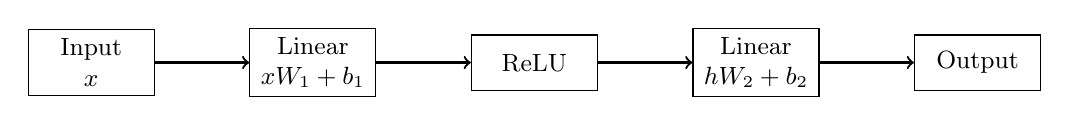
\begin{tikzpicture}[
    node distance=1.2cm,
    layer/.style={rectangle, draw, minimum width=1.6cm, minimum height=0.7cm, align=center, font=\small},
    arrow/.style={->, thick}
]
    \node[layer] (input) {Input\\$x$};
    \node[layer, right=of input] (linear1) {Linear\\$xW_1 + b_1$};
    \node[layer, right=of linear1] (relu) {ReLU};
    \node[layer, right=of relu] (linear2) {Linear\\$hW_2 + b_2$};
    \node[layer, right=of linear2] (output) {Output};

    \draw[arrow] (input) -- (linear1);
    \draw[arrow] (linear1) -- (relu);
    \draw[arrow] (relu) -- (linear2);
    \draw[arrow] (linear2) -- (output);
\end{tikzpicture}
\end{center}

The training loop repeats:
\begin{enumerate}
    \item \textbf{Forward pass}: Compute predictions from inputs
    \item \textbf{Loss computation}: Compare predictions to targets
    \item \textbf{Backward pass}: Compute gradients via \code{loss.backward()}
    \item \textbf{Parameter update}: Apply SGD step
    \item \textbf{Zero gradients}: Reset gradients for next iteration
\end{enumerate}

\begin{problembox}[mlp\_training]{Train a simple MLP on synthetic data \points{3}}

Implement an \code{MLP} class that:
\begin{itemize}
    \item Takes \code{input\_size}, \code{hidden\_size}, and \code{output\_size} as constructor arguments
    \item Creates two \code{Linear} layers: input$\to$hidden and hidden$\to$output
    \item In \code{\_\_call\_\_}: applies first linear, then ReLU, then second linear
    \item In \code{parameters()}: returns all parameters from both layers
\end{itemize}

The test will create synthetic classification data and verify that your MLP can be trained (loss decreases over iterations).

\deliverable{Implement the adapter \code{create\_mlp}, \code{run\_mlp}, and \code{get\_mlp\_parameters}. Run \code{uv run pytest -k TestMLP} to verify.}
\end{problembox}

\subsection{Interactive Demo}

Once your MLP is working, run the interactive demo to watch your neural network learn in real-time:

\begin{lstlisting}[style=bashstyle]
uv run python tests/cases/demo_mlp.py
\end{lstlisting}

This will train your MLP on a concentric circles dataset and show:
\begin{itemize}
    \item Real-time visualization of the decision boundary evolving
    \item Loss curve showing training progress
    \item Final performance summary
\end{itemize}

This is the reward for all your hard work---seeing your autodiff engine actually train a neural network!

\subsection{Numerical Gradient Checking}

Gradient checking verifies your analytical gradients by comparing them to numerical approximations. Using the central difference formula:
\begin{equation}
    \frac{\partial f}{\partial x_i} \approx \frac{f(x + h \cdot e_i) - f(x - h \cdot e_i)}{2h}
\end{equation}
where $e_i$ is a unit vector in the $i$-th direction and $h$ is a small value (e.g., $10^{-5}$).

\begin{problembox}[gradient\_check]{Implement gradient checking \points{2}}

Implement \code{check\_gradients(f, input, epsilon=1e-5, tolerance=1e-4)} that:
\begin{enumerate}
    \item Computes analytical gradients by calling \code{f(input)} and \code{backward()}
    \item Perturbs each element of the input tensor by $\pm\epsilon$ and computes numerical gradient
    \item Compares analytical and numerical gradients using relative error:
    \begin{equation}
        \text{rel\_error} = \frac{|g_{analytical} - g_{numerical}|}{\max(|g_{analytical}|, |g_{numerical}|) + \epsilon}
    \end{equation}
    \item Returns \code{True} if all relative errors are below the tolerance
\end{enumerate}

\textbf{Hint:} Flatten the tensor to iterate over elements, modify \code{data} directly when perturbing, and remember to restore the original value after each perturbation.

\deliverable{Implement the adapter \code{run\_gradient\_check}. Run \code{uv run pytest -k TestGradientCheck} to verify.}
\end{problembox}

\newpage
%==============================================================================
\section{Bonus: MNIST Handwritten Digit Recognition}
\points{5}
%==============================================================================

Train your autodiff engine on real handwritten digits from the MNIST dataset. This is the ultimate validation that your implementation works on a real machine learning benchmark with 60,000 training images.

\subsection{The Challenge}

MNIST is a dataset of 70,000 handwritten digits (0--9), each represented as a 28$\times$28 grayscale image. Your task:
\begin{itemize}
    \item Create an MLP with architecture: $784 \to \text{hidden} \to 10$
    \item Implement a training loop with mini-batch gradient descent
    \item Train on 60,000 images, test on 10,000 images
    \item Achieve $>$95\% test accuracy
\end{itemize}

We provide utility functions for loading and batching data. You implement the training.

\begin{problembox}[mnist\_training]{Train on MNIST handwritten digits \points{5}}

Implement the \code{train\_mnist} adapter function that:
\begin{enumerate}
    \item Creates an MLP suitable for MNIST (784 inputs, 10 outputs)
    \item Trains it using SGD with mini-batches
    \item Returns the trained model and final test accuracy
\end{enumerate}

\begin{lstlisting}[style=pythonsimple]
from smulgrad.engine import Tensor
from smulgrad.nn import MLP, softmax, cross_entropy, SGD
from tests.mnist_utils import load_mnist, mini_batch_iterator

def train_mnist(hidden_size, learning_rate, batch_size, epochs):
    train_X, train_y, test_X, test_y = load_mnist()

    # TODO: Create model

    # TODO: Training loop

    # TODO: Compute and return test accuracy
    return mlp, accuracy
\end{lstlisting}

\textbf{Grading:}
\begin{itemize}
    \item 3 points: Training loop works, loss decreases over epochs
    \item 2 points: Test accuracy $>$95\%
\end{itemize}

\deliverable{Implement the adapter \code{run\_mnist\_training} in \code{tests/adapters.py}. Run \code{uv run pytest -k TestMNIST} to verify.}

\end{problembox}

\subsection{Interactive Demo}

After completing this exercise, run the full interactive demo to visualize your network learning:

\begin{lstlisting}[style=bashstyle]
uv run python tests/cases/demo_mnist.py
\end{lstlisting}

This shows:
\begin{itemize}
    \item Sample digits from the training set
    \item Live training progress with loss and accuracy
    \item Training curves (loss and accuracy over epochs)
    \item Model predictions on test digits
    \item Comparison of correct vs incorrect predictions
\end{itemize}

\newpage
%==============================================================================
\section{Additional Bonus Challenges}
%==============================================================================

Once you've completed the main assignment and MNIST, try these extensions:

\subsection*{Bonus: More Optimizers \hfill 5 points}
Implement Adam optimizer with momentum and adaptive learning rates.

\subsection*{Bonus: Convolutional Operations \hfill 10 points}
Implement 2D convolution with correct gradients.

\subsection*{Bonus: Visualization \hfill 3 points}
Implement a function to visualize computational graphs using graphviz.

%==============================================================================
\section{Tips and Common Pitfalls}
%==============================================================================

\begin{enumerate}
    \item \textbf{Gradient accumulation}: When a value is used multiple times, gradients accumulate. Initialize gradients to 0 and use \code{+=} in backward.

    \item \textbf{Topological order}: Process nodes in reverse topological order during backward. A node's backward should only be called after all its consumers have been processed.

    \item \textbf{Broadcasting}: When shapes differ, numpy broadcasts. Your backward must ``unbroadcast'' by summing along the broadcasted dimensions.

    \item \textbf{Numerical stability}: In softmax and cross-entropy, subtract the maximum value before exponentiating to prevent overflow.

    \item \textbf{In-place operations}: Be careful with in-place numpy operations---they can corrupt gradient computation. Always create new arrays.

    \item \textbf{Zero gradients}: Remember to zero gradients before each backward pass, or they will accumulate across iterations.
\end{enumerate}

%==============================================================================
\section{References}
%==============================================================================

\begin{itemize}
    \item Karpathy's micrograd: \url{https://github.com/karpathy/micrograd}
    \item PyTorch autograd documentation: \url{https://pytorch.org/docs/stable/autograd.html}
    \item Stanford CS231n backpropagation notes: \url{https://cs231n.github.io/optimization-2/}
    \item Baydin et al., ``Automatic Differentiation in Machine Learning: a Survey''
\end{itemize}

\vspace{2em}
\begin{center}
    \textit{Good luck, and enjoy building your own autodiff engine!}
\end{center}

\end{document}
